\documentclass[a4paper,12pt]{article}
\usepackage[table]{xcolor}
\usepackage{array,amsmath,amssymb,multicol,tikz}
\usepackage{hyperref,colonequals}
\usepackage[margin=2cm]{geometry}
\usepackage{fancyvrb}
\usetikzlibrary{calc,arrows.meta}
\usepackage{xcolor}

\tikzset{
arr/.style={line width=1pt,-{Straight Barb[width=6pt, length=3pt]}, shorten >=2pt}
}

\pagestyle{empty}

\newcommand\N{\mathbf{N}}
\newcommand\Q{\mathbf{Q}}
\newcommand\R{\mathbf{R}}
\newcommand\Z{\mathbf{Z}}

\newcommand\rem{\textup{rem}}

\setlength{\parindent}{0pt}

\begin{document}

\begin{center}
\parbox{3cm}{\flushleft\bf Discrete\linebreak Structures}
\hfill
\parbox{7cm}{\centering {\bf\Huge Samples, Part 3}}
\hfill
\parbox{3cm}{\flushright\bf Spring 2021 \linebreak May 28}
\end{center}

\hrule\vspace{2pt}\hrule

\hrule


\vspace{10pt}
{\bf Combinatorics.}

\begin{enumerate}
% 1.(a)
\item {\small \em Given a word problem, count variants using the product, sum, difference rules.}\\
The following problem deals with English alphabet consisting of exactly $26$ letters (assume that
all letters are upper-case). Assume that there are $6$ vowels ({\tt A}, {\tt E}, {\tt I}, {\tt O}, {\tt U}, {\tt Y});
all the other $20$ letters are considered consonants.
\begin{enumerate}
\item A car license number in some city should consist of $4$ different letters; it should start with
two consonants followed by two vowels. How many license numbers are possible?
\item A car license number in some other city should consist of $4$ different letters;
two consonants and two vowels (in any order). How many license numbers are possible?
\item A car license number in some other city should consist of $4$ letters \textendash{} not necessarily different;
two consonants and two vowels (in any order). How many license numbers are possible?
\end{enumerate}


% 1.(b)
\item {\small \em Given a set of restrictions and symmetries, count variants using the division rule.}\\
Consider the following three situations and find the number of variants to complete each task:
\begin{enumerate}
\item In how many ways can we arrange $7$ bits in the following string: $\mathtt{0000111}$ (the order of bits matters;
the string must contain four 0s and three 1s).
\item There are $7$ seats enumerated with numbers $1,2,\ldots,7$. In how many ways can we seat three people on these seats
(the only thing that matters is \textendash{} which seats are occupied; it does not matter who is seated where).
\item A traveler needs to go from point $A$ to point $B$ in a city where there the streets are perpendicular and
all blocks have square shape as in Figure~\ref{fig:part3-square-city}. He should go three blocks to the north and four blocks to the east (extra circling around is
not allowed). In how many ways can he pick a route that leads from $A$ to $B$ following these rules?

\begin{figure}[!htb]
\center{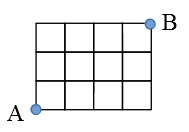
\includegraphics[width=1.2in]{figs/part3-square-city.png}}
\caption{\label{fig:part3-square-city}  City with points $A$ and $B$.}
\end{figure}

\begin{center}

\end{center}
\end{enumerate}


% 1.(c)
\item {\small \em Count variants using combinations and permutation formulas with or without repetition.}\\
Assume that we have $4$ different sorts of candy (and any two pieces of the same sort of candy are considered indistinguishable).
We want to create a set of $7$ candies; and there are no limitations on how many candies of each sort should be in the set.
\begin{enumerate}
\item How many sets of $7$ candies can be created, if the order of candies in the set (which candy is the first, which
is the second etc.) is important?
\item How many sets of $7$ candies can be created, if the order of candies in the set does not matter?
\end{enumerate}


% 1.(d)
\item {\small \em Given a polynomial, find coefficients using binomial and multinomial rules.}\\
Consider the following expression ${\displaystyle \left(x^2 - \frac{1}{x}\right)^{9}}$.
\begin{enumerate}
\item
How many terms are there in the expression  after we expand it using the binomial formula?
\item
Which term has the largest (positive) coefficient; find that term.
\end{enumerate}
\end{enumerate}





\vspace{10pt}
{\bf Recurrent Sequences.}

\begin{enumerate}
%2.(a)
\item {\small \em Evaluate $\sum\limits_{i=0}^n \ldots$ and similar constructs.}\\
Consider the following summation expression:
\[ \sum\limits_{k=1}^n \frac{3k + 5}{n^2}. \]
\begin{enumerate}
\item On what parameter(s) does this expression depend?
\item Rewrite it without using any summation symbols (or omissions with $\ldots$).
\end{enumerate}



%2.(b)
\item {\small \em Prove a property of a recurrent sequence by induction or using invariants.}\\
Let $F_0 = 0$, $F_1 = 1$, $F_n = F_{n-1} + F_{n-2}$ (for $n \geq 2$) be the Fibonacci sequence.
Prove by induction that every 5th member of this sequence is divisible by $5$.

%2.(c)
\item {\small \em Prove that a recurrent sequence has a closed formula using induction.}\\
Let $(a_n)$ be a sequence defined by this recurrence:
\[ \left\{ \begin{array}{l}
a_0 = 0,\\
a_{n} = a_{n-1} + \frac{1}{n(n+1)},\;\mbox{for $n \geq 1$}.
\end{array} \right. \]
Prove by induction that $a_n = 1 - \frac{1}{n+1}$ for each $n \geq 0$.



%2.(d)
\item {\small \em Given a 1st order non-homogeneous recurrence, solve it.}\\
Let $a_n = 3a_{n-1} +2^n$ be a recurrence. (Is it linear? Non-linear? Homogeneous? Non-homogeneous?)
\begin{enumerate}
\item Show that $a_n = -2^{n+1}$ satisfies this recurrence.
\item Find a solution for this recurrence when $a_0 = 1$.
\end{enumerate}


%2.(e)
\item {\small \em Given a 2nd order homogeneous recurrence, solve it.}\\
Solve the recurrence relation $a_n = a_{n-1} + 6a_{n-2}$ (for each $n \geq 2$), if $a_0 = 3$, $a_1 = 6$.


%2.(f)
\item {\small \em Given a word problem (sets of strings, Tower of Hanoi, tilings, etc.) build recurrences.}\\
Let $L_{n}$ denote the number of lobsters caught on year $n$ (where $n = 1,2,\ldots$).
We know that the number of lobsters caught in some year is the average of lobsters caught in the
two previous years.
\begin{enumerate}
\item Write the recurrence that the sequence $L_n$ must satisfy.
\item Write the characteristic equation for this recurrence.
\item ({\em Optionally.} Solve the recurrence and express $L_n$ for any $n$, if the number of lobsters caught in year
$1$ was $100000$, but the number of lobsters caught in year $2$ was $300000$.)
\end{enumerate}

\end{enumerate}


%\clearpage
\vspace{10pt}
{\bf Big-O notation.}


\begin{enumerate}
%3.(a)
\item {\small \em Given functions $f,g$, check by definition that $f(n)$ is in $O(g(n))$, $\Omega(g(n))$, $\Theta(g(n))$.}\\
Check or disprove the possible relations between functions $f$ and $g$ (are they one another's Big-O, Big-Omega or Big-Theta), if the
functions are the following:
\begin{enumerate}
\item $f(n) = 0$, $g(n) = 17$.
\item $f(n) = 1.01^{100}$, $g(n) = n^{100}$.
\item $f(n) = 0.99^{100}$, $g(n) = n^{100}$.
\item $f(n) = 1 + \cos\left( \frac{\pi n}{2}\right)$ and  $g(n) = 1 + \sin\left( \frac{\pi n}{2}\right)$
\item $f(n) = \log_2 n$, $g(n) = \log_{10} n$.
\end{enumerate}

%3.(b)
\item {\small \em Given a function $f(x)$, simplify it to get its ``optimal'' $O(g(x))$ or $\Theta(g(x))$ class.}\\
Let $f(x) = \log_2 x + \log_2^2 x + \log_2 x^2$. Find a short (preferably one-term) expression $g(x)$ such
that $f(x)$ is in $\Theta(g(x))$.

%3.(c)
\item {\small \em Given a collection of functions, arrange them by growth.}\\
Given these functions: $\sqrt{n},\;\;1000 \log_2 n,\;\;n \log_2 n,\;\;2n!,\;\;(2n)!,\;\;2^n,\;\;\frac{n^2}{1000}$
arrange them in a sequence $f_1(n), f_2(n), \ldots$ so that $f_1(n)$ is in $O(f_2(n))$,
$f_2(n)$ is in $O(f_3(n))$ and so on. (Intuitively, every next function must asymptotically grow faster than the previous one.)


%3.(d)
\item {\small \em Given a pseudocode, basic operations and input length, estimate its time as $O(g(n))$.}\\
Figure~\ref{fig:part3-big-o-pseudocode} shows pseudocode. Find its worst-case time complexity in terms of $n$.
\begin{figure}[!htb]
\center{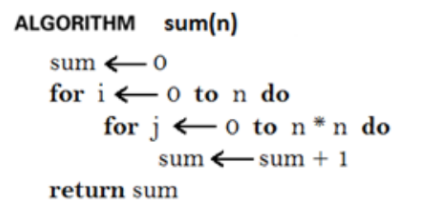
\includegraphics[width=3in]{figs/part3-big-o-pseudocode.png}}
\caption{\label{fig:part3-big-o-pseudocode}} Pseudocode for time complexity.
\end{figure}

\end{enumerate}



\end{document}
